% xelatex

\documentclass[12pt]{article}

\usepackage{enumitem}
\usepackage{amsmath}
\usepackage{amsfonts}
\usepackage{graphicx,color}    % on a mac

\usepackage{listings,boxedminipage}

\setlength{\topmargin}{-0.5in}

\setlength{\textheight}{9.0in}
\setlength{\textwidth}{7.5in}
\setlength{\oddsidemargin}{-0.5in}
%\setlength{\evensidemargin}{-0.1in}
\setlength{\parindent}{0mm}
\setlength{\parskip}{0.1in}

\newcommand{\forget}[1]{}
% new itemize environment with itemsep parameter
\newenvironment{myitemize}[1][0]
  { \begin{itemize}
    % set spacing between items
    \addtolength{\itemsep}{#1\baselineskip}
    % set spacing between lines
    \addtolength{\baselineskip}{#1\baselineskip} }
  { \end{itemize} }

\newenvironment{myenumerate}[1][0]
  { \begin{enumerate}
    % set spacing between items
    \addtolength{\itemsep}{#1\baselineskip}
    % set spacing between lines
    \addtolength{\baselineskip}{#1\baselineskip} }
  { \end{enumerate} }


\pagestyle{empty}
%\pagenumbering{nopagenumbering}

%\thispagestyle{empty}
\begin{document}

\title{\vspace{20ex}CS4450/7450 Midterm\\Fall 2016}
\date{October 10, 2016}


\maketitle
\thispagestyle{empty}

{\large
\begin{center}
\begin{minipage}{4.5in}
\begin{itemize}
\item This is a closed book, closed note exam.
\item You may not use a calculator or similar device.
\item Write all work on the exam itself.
\item There are 25 problems, each worth 4 points.
\end{itemize}
\vfill
\begin{tabbing}
{\bf Name:}\\\\
{\bf Pawprint:}
\end{tabbing}
\end{minipage}
\end{center}
}

\pagebreak

%%%%%%%%%%%%%%%%%%%%%%%%%%%%%%%%%%%%%%%%%%%%%%%
%%%%%%%%%%%%%%%%%%%%%%%%%%%%%%%%%%%%%%%%%%%%%%%
%%%%%%%%%%%%%%%%%%%%%%%%%%%%%%%%%%%%%%%%%%%%%%%
%%%%%%%%%%%%%%%%%%%%%%%%%%%%%%%%%%%%%%%%%%%%%%%
%%%%%%%%%%%%%%%%%%%%%%%%%%%%%%%%%%%%%%%%%%%%%%%

\noindent
{\bf {\textsc Part I.} 24 points total, 4 points each}.

\noindent
Indicate True or False in the following questions.



\begin{enumerate}[resume]
\item True or False. The following definition is valid (i.e., it does not cause an error
when loaded into the GHCi interpreter):
\begin{verbatim}
p1_1 :: (Int -> Int) -> Int -> Int
p1_1 _ _ = 9
\end{verbatim}
\item True or False. The following definition is valid:
\begin{verbatim}
p1_2 :: (Int -> Int) -> Int -> Int
p1_2 f x = 9
\end{verbatim}
\item True or False. The following definition is valid:
\begin{verbatim}
p1_3 :: (Int -> Int) -> Int -> Int
p1_3 f x = x
\end{verbatim}
\item True or False. The following definition is valid:
\begin{verbatim}
p1_4 :: (Int -> Int) -> Int -> Int
p1_4 f x = f (f (f x))
\end{verbatim}

\item True or False. The functions \verb+lf1+, \verb+lf2+, \verb+lf3+, and \verb+lf4+ are identical functions.
\begin{verbatim}
lf1 = map (\ x -> x)

lf2 = \ x -> x

lf3 []     = []
lf3 (x:xs) = x : lf3 xs

lf4 = foldr (:) []
\end{verbatim}
\end{enumerate}

%%%%%%%%%%%%%%%%%%%%%%%%%%%%%%%%%%%%%%%%%%%%%%%
%%%%%%%%%%%%%%%%%%%%%%%%%%%%%%%%%%%%%%%%%%%%%%%
%%%%%%%%%%%%%%%%%%%%%%%%%%%%%%%%%%%%%%%%%%%%%%%
%%%%%%%%%%%%%%%%%%%%%%%%%%%%%%%%%%%%%%%%%%%%%%%
%%%%%%%%%%%%%%%%%%%%%%%%%%%%%%%%%%%%%%%%%%%%%%%
\pagebreak


\begin{enumerate}[resume]
\item The following definition of a tree data type is similar to the one we saw in lecture:
\begin{verbatim}
       data Tree = Leaf Int | Node Tree Int Tree
\end{verbatim}
Define a value of type \verb+Tree+ corresponding to the diagram:
\begin{center}
\begin{boxedminipage}{1.9in}
\scalebox{0.35}{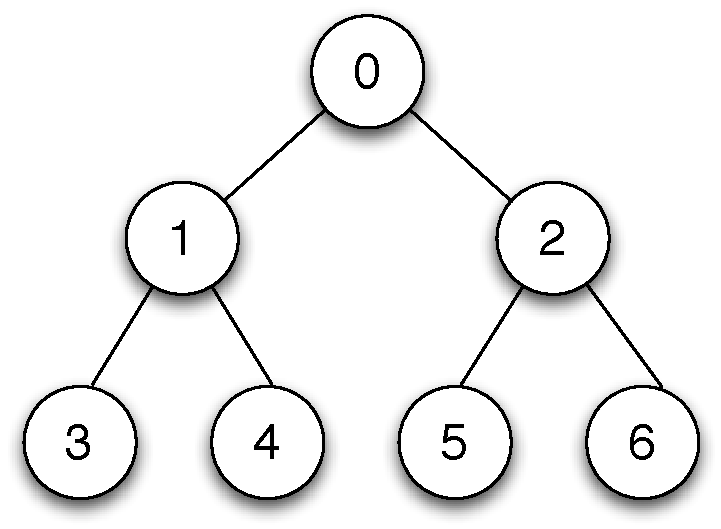
\includegraphics[]{tree}}
\end{boxedminipage}
\end{center}
\begin{verbatim}


t :: Tree
t = 
\end{verbatim}

\end{enumerate}

%%%%%%%%%%%%%%%%%%%%%%%%%%%%%%%%%%%%%%%%%%%%%%%
%%%%%%%%%%%%%%%%%%%%%%%%%%%%%%%%%%%%%%%%%%%%%%%
%%%%%%%%%%%%%%%%%%%%%%%%%%%%%%%%%%%%%%%%%%%%%%%
%%%%%%%%%%%%%%%%%%%%%%%%%%%%%%%%%%%%%%%%%%%%%%%
%%%%%%%%%%%%%%%%%%%%%%%%%%%%%%%%%%%%%%%%%%%%%%%
\pagebreak

\noindent
{\bf {\textsc Part II.} 36 points total, 4 points each}.

\noindent
Consider the following data type for representing the natural numbers:
\begin{verbatim}
       data Nat = Zero | Succ Nat
\end{verbatim}

For example, we can use this data type to represent the first few numerals
thusly:
%\begin{align*}
%0 &\equiv \text{\tt Zero}\\
%1 &\equiv \text{\tt Succ Zero}\\
%2 &\equiv \text{\tt Succ (Succ Zero)}\\
%\vdots
%\end{align*}
\begin{align*}
\text{\tt Zero} &\text{ stands for } 0 \\
\text{\tt Succ Zero} &\text{ stands for } 1 \\
\text{\tt Succ (Succ Zero)} &\text{ stands for }  2 \\
\vdots
\end{align*}
Given this, what operation do the following Haskell definitions implement?
Choose the best answer.

\begin{enumerate}[resume]
\item \begin{verbatim}
(<?>) :: Nat -> Nat -> Nat
a <?> Zero            = a
(Succ a) <?> (Succ n) = a <?> n
\end{verbatim}
\begin{enumerate}
\item Addition.
\item Subtraction.
\item Multiplication.
\item Integer division.
\item Exponentiation (i.e., $x^y$).
\end{enumerate}

\item Where {\tt (*) :: Nat -> Nat -> Nat} is multiplication,
\begin{verbatim}
(<?>) :: Nat -> Nat -> Nat
n <?> Zero     = Succ Zero
n <?> (Succ m) = n * (n <?> m)
\end{verbatim}
\begin{enumerate}
\item Addition.
\item Subtraction.
\item Multiplication.
\item Integer division.
\item Exponentiation.
\end{enumerate}

\pagebreak

\item \begin{verbatim}
(<?>) :: Nat -> Nat -> Nat
Zero <?> a     = a
(Succ n) <?> a = Succ (n <?> a)
\end{verbatim}
\begin{enumerate}
\item Addition.
\item Subtraction.
\item Multiplication.
\item Integer division.
\item Exponentiation.
\end{enumerate}

\item Where {\tt (-) :: Nat -> Nat -> Nat} is subtraction,
\begin{verbatim}
(<?>) :: Nat -> Nat -> Nat
Zero <?> a = Zero
n <?> a    = foo Zero n a

foo :: Nat -> Nat -> Nat -> Nat
foo acc n a | n < a     = acc
            | otherwise = foo (Succ acc) (n - a) a
\end{verbatim}
\begin{enumerate}
\item Addition.
\item Subtraction.
\item Multiplication.
\item Integer division.
\item Exponentiation.
\end{enumerate}

\item Where {\tt (+) :: Nat -> Nat -> Nat} is addition,
\begin{verbatim}
(<?>) :: Nat -> Nat -> Nat
Zero <?> a     = Zero
(Succ n) <?> a = a + (n <?> a)
\end{verbatim}
\begin{enumerate}
\item Addition.
\item Subtraction.
\item Multiplication.
\item Integer division.
\item Exponentiation.
\end{enumerate}

\pagebreak

\item \begin{verbatim}
(<?>) :: Nat -> Nat -> Bool
Zero <?> Zero         = True
Zero <?> (Succ n)     = True
(Succ n) <?> (Succ m) = n <?> m
x <?> z               = False
\end{verbatim}
\begin{enumerate}
\item Equality (i.e., $x == y$).
\item Less than (i.e., $x < y$).
\item Less than or equal (i.e., $x \leq y$).
\item Greater than (i.e., $x > y$).
\item Greater than or equal (i.e. $x \geq y$).
\end{enumerate}

\item \begin{verbatim}
(<?>) :: Nat -> Nat -> Bool
(Succ n) <?> Zero     = True
(Succ n) <?> (Succ m) = n <?> m
x <?> z               = False
\end{verbatim}
\begin{enumerate}
\item Equality.
\item Less than.
\item Less than or equal.
\item Greater than.
\item Greater than or equal.
\end{enumerate}

\item \begin{verbatim}
(<?>) :: Nat -> Nat -> Bool
Zero <?> Zero         = True
(Succ n) <?> Zero     = True
(Succ n) <?> (Succ m) = n <?> m
x <?> z               = False
\end{verbatim}
\begin{enumerate}
\item Equality.
\item Less than.
\item Less than or equal.
\item Greater than.
\item Greater than or equal.
\end{enumerate}

\pagebreak

%\item \begin{verbatim}
%(<?>) :: Nat -> Nat -> Bool
%Zero <?> (Succ n)     = True
%(Succ n) <?> (Succ m) = n <?> m
%z <?> x               = False
%\end{verbatim}
%\begin{enumerate}
%\item Equality.
%\item Less than.
%\item Less than or equal.
%\item Greater than.
%\item Greater than or equal.
%\end{enumerate}

\item \begin{verbatim}
(<?>) :: Nat -> Nat -> Bool
Zero <?> Zero         = True
(Succ n) <?> (Succ m) = n <?> m
z <?> x               = False
\end{verbatim}
\begin{enumerate}
\item Equality.
\item Less than.
\item Less than or equal.
\item Greater than.
\item Greater than or equal.
\end{enumerate}

\end{enumerate}

\pagebreak

\noindent
{\bf {\textsc Part III.} 40 points total, 4 points each}.

\noindent
Choose the correct type annotation for the following Haskell definitions.

\begin{enumerate}[resume]
\item \begin{verbatim}
f1 f x y = f (x,y)
\end{verbatim}
\begin{enumerate}
\item {\tt f1 :: (t1 -> t2 -> t) -> (t1, t2) -> t}
\item {\tt f1 :: ((t1, t2) -> t) -> t1 -> t2 -> t}
\item {\tt f1 :: (t1, t2) -> t -> t1 -> t2 -> t}
\item {\tt f1 :: t1 -> t2 -> t -> t1 -> t2 -> t}
\end{enumerate}

\item \begin{verbatim}
f2 f (x,y) = f x y
\end{verbatim}
\begin{enumerate}
\item {\tt f2 :: (t1 -> t2 -> t) -> (t1, t2) -> t}
\item {\tt f2 :: ((t1, t2) -> t) -> t1 -> t2 -> t}
\item {\tt f2 :: ((t1,t2) -> t) -> (t1, t2) -> t}
\item {\tt f2 :: (t1 -> t2 -> t) -> (t1, t2) -> t}
\end{enumerate}

\item \begin{verbatim}
f3 f x y = f y x
\end{verbatim}
\begin{enumerate}
\item {\tt f3 :: (t1 -> t2 -> t) -> t2 -> t1 -> t}
\item {\tt f3 :: t2 -> t1 -> (t1 -> t2 -> t) -> t}
\item {\tt f3 :: ((t1, t2) -> t) -> t2 -> t1 -> t}
\item {\tt f3 :: ((t1, t2) -> t) -> (t2, t1) -> t}
\end{enumerate}

\item \begin{verbatim}
f4 [x,y] = x
\end{verbatim}
\begin{enumerate}
\item {\tt f4 :: [t] -> t}
\item {\tt f4 :: (t,t) -> t}
\item {\tt f4 :: (t,t1) -> t}
\item {\tt f4 :: (t1,t) -> t}
\end{enumerate}

\item \begin{verbatim}
f5 (x,y) = (x,x)
\end{verbatim}
\begin{enumerate}
\item {\tt f5 :: (t, t1) -> (t1, t1)}
\item {\tt f5 :: (t1, t) -> (t, t1)}
\item {\tt f5 :: (t1, t) -> (t1, t1)}
\item None of the above.
%\item {\tt f5 :: (t, t) -> (t, t)}
\end{enumerate}

\item \begin{verbatim}
data Either a b = Left a | Right b
data Maybe a    = Just a | Nothing

f6 (Left x)  = Just x
f6 (Right y) = Nothing
\end{verbatim}
\begin{enumerate}
\item {\tt f6 :: Either a a -> Maybe a}
\item {\tt f6 :: Either t a -> Maybe a}
\item {\tt f6 :: Either a t -> Maybe a}
\item None of the above.
\end{enumerate}

\item \begin{verbatim}
f7 (Just x) = Left x
f7 Nothing  = Right undefined
\end{verbatim}
\begin{enumerate}
\item {\tt f7 :: Maybe a -> Either b a}
\item {\tt f7 :: Maybe a -> Either a b}
\item All of the above.
\item None of the above.
\end{enumerate}

\item \begin{verbatim}
f8 (Left x)  = Left (Just x)
f8 (Right x) = Right Nothing
\end{verbatim}
\begin{enumerate}
\item {\tt f8 :: Either a t -> Either (Maybe a) (Maybe a1)}
\item {\tt f8 :: Either a a1 -> Either (Maybe a) (Maybe a1)}
\item {\tt f8 :: Either a a1 -> Either (Maybe a1) (Maybe a)}
\item None of the above.
\end{enumerate}

\item \begin{verbatim}
f9 (x,y) = (y,x)
\end{verbatim}
\begin{enumerate}
\item {\tt f9 :: (t1, t) -> (t1, t)}
\item {\tt f9 :: (t1, t) -> (t, t1)}
\item {\tt f9 :: (t, t) -> (t, t1)}
\item None of the above.
\end{enumerate}

\item \begin{verbatim}
f10 x = \ s -> (x,s)
\end{verbatim}
\begin{enumerate}
\item {\tt f10 :: t -> t1 -> (t, t1)}
\item {\tt f10 :: (t, t1) -> (t, t1)}
\item {\tt f10 :: (t1, t1) -> t -> t1}
\item {\tt None of the above.}
\end{enumerate}

\end{enumerate}

\end{document}

